\documentclass[11pt]{article}
\usepackage[margin=1in]{geometry}
\usepackage{booktabs}
\usepackage{longtable}
\usepackage{array}
\usepackage{siunitx}
\usepackage{pgfplots}
\usepackage{tikz}
\usepackage{hyperref}
\pgfplotsset{compat=1.18}
\sisetup{group-separator={,}, round-mode=places, round-precision=2}

\title{RailGuard Health: 5-Year SaaS Financial Model Inputs\\(SmartHelping Template Ready)}
\author{CSC454 Assignment 5}
\date{March 13, 2026}

\begin{document}
\maketitle

\noindent\textbf{Currency:} CAD unless noted. \textbf{Market focus:} Canada first, US expansion starting Year 4. \textbf{Model posture:} venture-backed, aggressive growth, moderate healthcare sales cycle.

\section*{1. Core Financial Assumptions}
\begin{longtable}{p{0.38\textwidth} p{0.16\textwidth} p{0.40\textwidth}}
\toprule
\textbf{Variable} & \textbf{Value} & \textbf{Justification} \\
\midrule
Monthly blended ARPU (Y1--Y5) & 244, 259, 274, 287, 299 & Falls inside AI scribe market range; increases as billing/compliance features and enterprise controls expand. \\
Average providers per clinic & 4.2 & Matches target of small/medium outpatient clinics (1--10 clinicians). \\
Monthly logo churn & 1.8\% (Y1), 1.6\% (Y2), 1.4\% (Y3+)& Sticky workflow software once embedded into EMR operations. \\
Gross margin target & 80\%+ by Y3 & Healthcare SaaS target with improving inference efficiency and stable hosting costs. \\
CAC per new provider & 2,000 (Y1) down to 1,167 (Y4) & EMR-linked sales requires pilots and implementation support early, then referral and partner leverage. \\
Implementation fee per new clinic & 1,500 (Y1--Y2), 2,000 (Y3--Y5) & One-time onboarding/training/configuration revenue. \\
Sales cycle length & 2--4 months & Typical for outpatient clinics buying compliance-sensitive software. \\
Capex & 180k, 220k, 280k, 350k, 420k & Security, platform reliability, and analytics infrastructure scaling. \\
\bottomrule
\end{longtable}

\section*{2. Customer Growth Model (Providers Subscribed)}
\begin{center}
\begin{tabular}{lrrrr}
\toprule
\textbf{Year} & \textbf{Clinics (EOY)} & \textbf{Providers (EOY)} & \textbf{Providers (Avg Active)} & \textbf{Provider Growth} \\
\midrule
Y1 & 22 & 90 & 70 & -- \\
Y2 & 76 & 320 & 260 & 255.6\% \\
Y3 & 214 & 900 & 760 & 181.3\% \\
Y4 & 500 & 2,100 & 1,850 & 133.3\% \\
Y5 & 980 & 4,200 & 3,700 & 100.0\% \\
\bottomrule
\end{tabular}
\end{center}

\noindent\textbf{Adoption drivers:} (1) EMR marketplace visibility and integrations, (2) physician referrals from pilot clinics, (3) faster onboarding playbooks by Y3, (4) US partner channels starting Y4.

\begin{figure}[h]
\centering
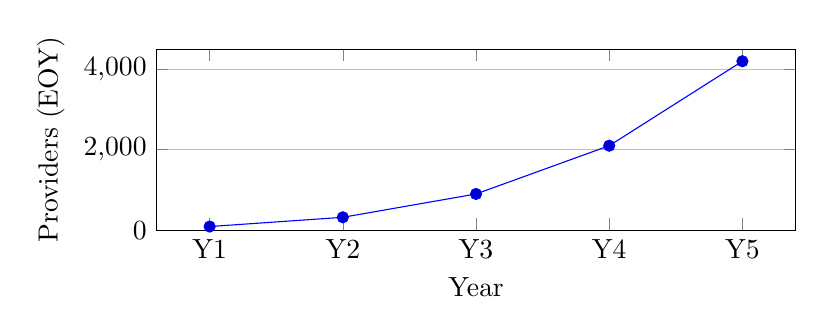
\begin{tikzpicture}
\begin{axis}[
    width=0.8\textwidth,
    height=0.32\textwidth,
    xlabel={Year},
    ylabel={Providers (EOY)},
    symbolic x coords={Y1,Y2,Y3,Y4,Y5},
    xtick=data,
    ymin=0,
    ymax=4500,
    ymajorgrids=true
]
\addplot+[mark=*] coordinates {(Y1,90) (Y2,320) (Y3,900) (Y4,2100) (Y5,4200)};
\end{axis}
\end{tikzpicture}
\caption{Provider Growth Trajectory}
\end{figure}

\section*{3. Pricing Model}
\begin{center}
\begin{tabular}{p{0.2\textwidth} p{0.2\textwidth} p{0.5\textwidth}}
\toprule
\textbf{Plan} & \textbf{Price (per provider/month)} & \textbf{Key Features} \\
\midrule
Basic & 199 & Transcription, structured notes, EMR write-back \\
Professional & 299 & Billing optimization, coding support, compliance validation \\
Enterprise & 399 & Advanced analytics, admin controls, multi-site governance \\
\bottomrule
\end{tabular}
\end{center}

\begin{center}
\begin{tabular}{lcc}
\toprule
\textbf{Year} & \textbf{Plan Mix (B/P/E)} & \textbf{Blended ARPU} \\
\midrule
Y1 & 60\% / 35\% / 5\% & 244 \\
Y2 & 50\% / 40\% / 10\% & 259 \\
Y3 & 40\% / 45\% / 15\% & 274 \\
Y4 & 32\% / 48\% / 20\% & 287 \\
Y5 & 25\% / 50\% / 25\% & 299 \\
\bottomrule
\end{tabular}
\end{center}

\section*{4. Revenue Projections}
\[
\text{Annual Revenue} = (\text{Avg Active Providers} \times \text{ARPU} \times 12) + \text{Implementation Fees}
\]

\begin{center}
\begin{tabular}{lrrrr}
\toprule
\textbf{Year} & \textbf{Avg Providers} & \textbf{ARPU} & \textbf{Subscription Revenue} & \textbf{Total Revenue} \\
\midrule
Y1 & 70 & 244 & 204,960 & 234,960 \\
Y2 & 260 & 259 & 808,080 & 888,080 \\
Y3 & 760 & 274 & 2,498,880 & 2,718,880 \\
Y4 & 1,850 & 287 & 6,368,400 & 6,868,400 \\
Y5 & 3,700 & 299 & 13,275,600 & 14,275,600 \\
\bottomrule
\end{tabular}
\end{center}

\begin{figure}[h]
\centering
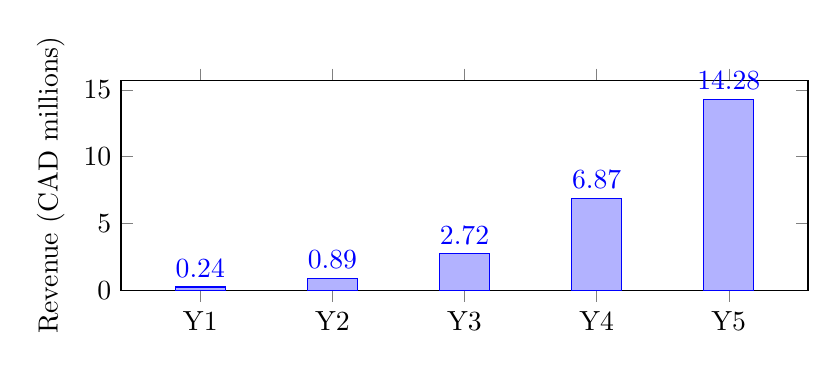
\begin{tikzpicture}
\begin{axis}[
    width=0.85\textwidth,
    height=0.35\textwidth,
    ybar,
    bar width=18pt,
    ylabel={Revenue (CAD millions)},
    symbolic x coords={Y1,Y2,Y3,Y4,Y5},
    xtick=data,
    nodes near coords,
    ymin=0,
    enlarge x limits=0.15
]
\addplot coordinates {(Y1,0.235) (Y2,0.888) (Y3,2.719) (Y4,6.868) (Y5,14.276)};
\end{axis}
\end{tikzpicture}
\caption{Total Revenue Growth}
\end{figure}

\section*{5. Cost of Goods Sold (COGS)}
\begin{center}
\begin{tabular}{p{0.5\textwidth} r}
\toprule
\textbf{Cost Component} & \textbf{Cost per Provider / Month} \\
\midrule
LLM inference and clinical summarization & 24 \\
Cloud hosting and networking & 11 \\
Storage, audit logs, and security retention & 5 \\
Support and implementation servicing & 8 \\
Payment processing and marketplace fees & 6 \\
\midrule
\textbf{Total COGS per provider / month} & \textbf{54} \\
\bottomrule
\end{tabular}
\end{center}

\begin{center}
\begin{tabular}{lrrr}
\toprule
\textbf{Year} & \textbf{Revenue} & \textbf{COGS} & \textbf{Gross Margin} \\
\midrule
Y1 & 234,960 & 45,360 & 80.7\% \\
Y2 & 888,080 & 168,480 & 81.0\% \\
Y3 & 2,718,880 & 492,480 & 81.9\% \\
Y4 & 6,868,400 & 1,198,800 & 82.5\% \\
Y5 & 14,275,600 & 2,397,600 & 83.2\% \\
\bottomrule
\end{tabular}
\end{center}

\section*{6. 5-Year Hiring Plan}
\begin{center}
\begin{tabular}{lrrrrrr}
\toprule
\textbf{Role} & \textbf{Salary} & \textbf{Y1} & \textbf{Y2} & \textbf{Y3} & \textbf{Y4} & \textbf{Y5} \\
\midrule
Leadership/Ops & 180k & 2 & 2 & 2 & 2 & 2 \\
Backend/Platform Engineer & 135k & 2 & 2 & 5 & 6 & 7 \\
ML Engineer & 145k & 1 & 2 & 3 & 3 & 4 \\
Clinical AI Specialist & 125k & 1 & 1 & 1 & 2 & 2 \\
Product Manager & 140k & 0 & 1 & 1 & 2 & 3 \\
Compliance/Privacy Officer & 120k & 0 & 1 & 1 & 1 & 2 \\
Sales/Partnerships (OTE) & 130k & 0 & 0 & 1 & 3 & 6 \\
Customer Success/Implementation & 95k & 0 & 1 & 2 & 5 & 7 \\
\midrule
\textbf{Total FTE} & -- & \textbf{6} & \textbf{10} & \textbf{16} & \textbf{24} & \textbf{33} \\
\bottomrule
\end{tabular}
\end{center}

\noindent\textbf{Hiring logic:} engineering-heavy through Y3 for integrations and model reliability, then GTM and customer success expansion in Y4--Y5 to scale clinic acquisition and retention.

\section*{7. Operating Expenses (Non-COGS, Non-Payroll)}
\begin{center}
\begin{tabular}{lrrrrr}
\toprule
\textbf{Category} & \textbf{Y1} & \textbf{Y2} & \textbf{Y3} & \textbf{Y4} & \textbf{Y5} \\
\midrule
Marketing and demand generation & 180,000 & 320,000 & 700,000 & 1,400,000 & 2,700,000 \\
Legal and compliance & 60,000 & 80,000 & 110,000 & 170,000 & 250,000 \\
Conferences and travel & 20,000 & 40,000 & 70,000 & 120,000 & 180,000 \\
SaaS tools and software ops & 45,000 & 65,000 & 95,000 & 140,000 & 190,000 \\
Infrastructure overhead (non-COGS) & 40,000 & 55,000 & 85,000 & 130,000 & 180,000 \\
Insurance and admin overhead & 23,000 & 30,000 & 45,000 & 70,000 & 95,000 \\
\midrule
\textbf{Total Non-Payroll Opex} & \textbf{368,000} & \textbf{590,000} & \textbf{1,105,000} & \textbf{2,030,000} & \textbf{3,595,000} \\
\bottomrule
\end{tabular}
\end{center}

\section*{8. CAC Payback}
\[
\text{CAC Payback (months)} = \frac{\text{CAC per new provider}}{\text{Monthly Gross Profit per provider}}
\]
\[
\text{Monthly Gross Profit per provider} = \text{ARPU} - \text{COGS per provider/month}
\]

\begin{center}
\begin{tabular}{lrrrr}
\toprule
\textbf{Year} & \textbf{CAC / New Provider} & \textbf{ARPU} & \textbf{Monthly Gross Profit} & \textbf{Payback (months)} \\
\midrule
Y1 & 2,000 & 244 & 190 & 10.5 \\
Y2 & 1,391 & 259 & 205 & 6.8 \\
Y3 & 1,207 & 274 & 220 & 5.5 \\
Y4 & 1,167 & 287 & 233 & 5.0 \\
Y5 & 1,286 & 299 & 245 & 5.2 \\
\bottomrule
\end{tabular}
\end{center}

\begin{figure}[h]
\centering
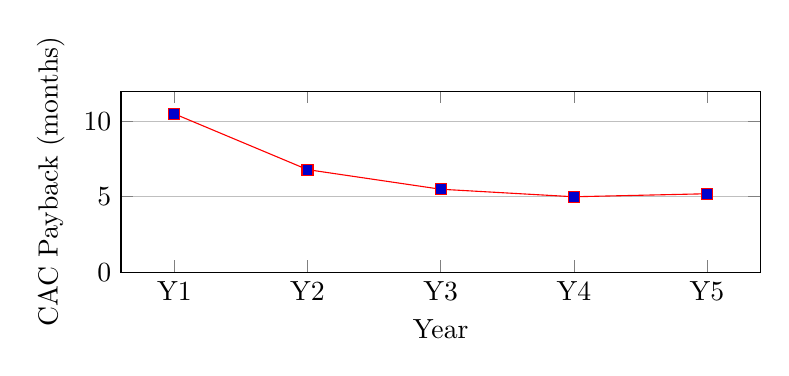
\begin{tikzpicture}
\begin{axis}[
    width=0.8\textwidth,
    height=0.32\textwidth,
    xlabel={Year},
    ylabel={CAC Payback (months)},
    symbolic x coords={Y1,Y2,Y3,Y4,Y5},
    xtick=data,
    ymin=0,
    ymax=12,
    ymajorgrids=true
]
\addplot+[mark=square*, color=red] coordinates {(Y1,10.5) (Y2,6.8) (Y3,5.5) (Y4,5.0) (Y5,5.2)};
\end{axis}
\end{tikzpicture}
\caption{CAC Payback Improvement}
\end{figure}

\section*{9. Break-Even Analysis}
\begin{center}
\begin{tabular}{lrrrrr}
\toprule
\textbf{Year} & \textbf{Revenue} & \textbf{COGS} & \textbf{SG\&A} & \textbf{EBITDA} & \textbf{EBITDA Margin} \\
\midrule
Y1 & 234,960 & 45,360 & 1,250,000 & -1,060,400 & -451.3\% \\
Y2 & 888,080 & 168,480 & 1,950,000 & -1,230,400 & -138.5\% \\
Y3 & 2,718,880 & 492,480 & 3,100,000 & -873,600 & -32.1\% \\
Y4 & 6,868,400 & 1,198,800 & 4,900,000 & 769,600 & 11.2\% \\
Y5 & 14,275,600 & 2,397,600 & 7,100,000 & 4,778,000 & 33.5\% \\
\bottomrule
\end{tabular}
\end{center}

\noindent\textbf{Break-even point:} EBITDA turns positive in \textbf{Year 4}.\\
\textbf{Sensitivity:} if provider adoption is 20\% lower than plan, break-even shifts from Y4 to Y5. If ARPU is 10\% below plan, CAC payback worsens by roughly 0.7--1.0 months.

\begin{figure}[h]
\centering
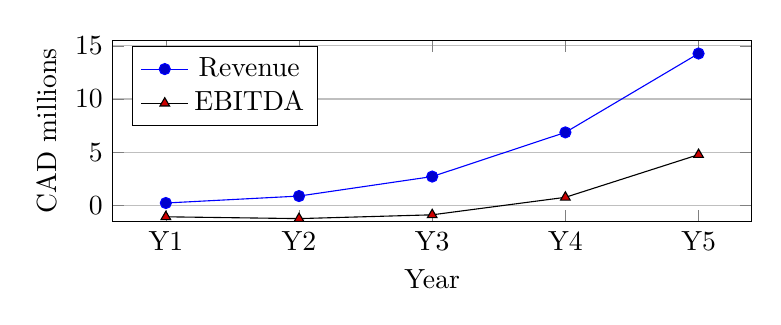
\begin{tikzpicture}
\begin{axis}[
    width=0.8\textwidth,
    height=0.32\textwidth,
    xlabel={Year},
    ylabel={CAD millions},
    symbolic x coords={Y1,Y2,Y3,Y4,Y5},
    xtick=data,
    ymin=-1.5,
    ymax=15.5,
    ymajorgrids=true,
    legend pos=north west
]
\addplot+[mark=*, color=blue] coordinates {(Y1,0.235) (Y2,0.888) (Y3,2.719) (Y4,6.868) (Y5,14.276)};
\addplot+[mark=triangle*, color=black] coordinates {(Y1,-1.060) (Y2,-1.230) (Y3,-0.874) (Y4,0.770) (Y5,4.778)};
\legend{Revenue, EBITDA}
\end{axis}
\end{tikzpicture}
\caption{Revenue vs EBITDA}
\end{figure}

\begin{figure}[h]
\centering
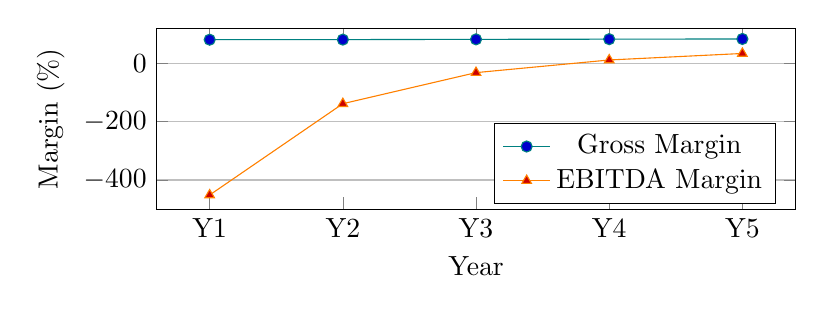
\begin{tikzpicture}
\begin{axis}[
    width=0.8\textwidth,
    height=0.32\textwidth,
    xlabel={Year},
    ylabel={Margin (\%)},
    symbolic x coords={Y1,Y2,Y3,Y4,Y5},
    xtick=data,
    ymin=-500,
    ymax=120,
    ymajorgrids=true,
    legend pos=south east
]
\addplot+[mark=*, color=teal] coordinates {(Y1,80.7) (Y2,81.0) (Y3,81.9) (Y4,82.5) (Y5,83.2)};
\addplot+[mark=triangle*, color=orange] coordinates {(Y1,-451.3) (Y2,-138.5) (Y3,-32.1) (Y4,11.2) (Y5,33.5)};
\legend{Gross Margin, EBITDA Margin}
\end{axis}
\end{tikzpicture}
\caption{Gross Margin vs EBITDA Margin}
\end{figure}

\begin{figure}[h]
\centering
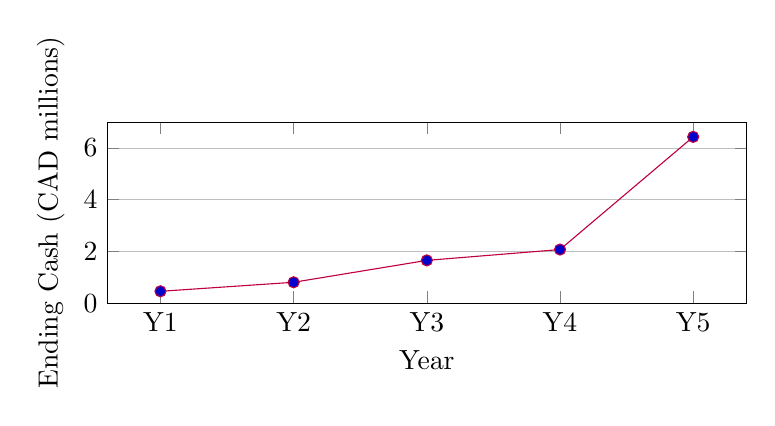
\begin{tikzpicture}
\begin{axis}[
    width=0.8\textwidth,
    height=0.32\textwidth,
    xlabel={Year},
    ylabel={Ending Cash (CAD millions)},
    symbolic x coords={Y1,Y2,Y3,Y4,Y5},
    xtick=data,
    ymin=0,
    ymax=7,
    ymajorgrids=true
]
\addplot+[mark=*, color=purple] coordinates {(Y1,0.460) (Y2,0.809) (Y3,1.656) (Y4,2.075) (Y5,6.433)};
\end{axis}
\end{tikzpicture}
\caption{Cash Balance Over Time}
\end{figure}

\section*{10. SmartHelping Excel Template Mapping}
\begin{center}
\begin{tabular}{p{0.46\textwidth} p{0.42\textwidth}}
\toprule
\textbf{Template Section} & \textbf{Input Value to Enter} \\
\midrule
Pricing assumptions (monthly ARPU) & 244, 259, 274, 287, 299 by year \\
Subscriber growth assumptions & Avg providers: 70, 260, 760, 1,850, 3,700 \\
New subscribers for CAC sheet & 90, 230, 580, 1,200, 2,100 \\
Monthly churn assumption & 1.8\%, 1.6\%, 1.4\%, 1.4\%, 1.4\% \\
COGS per subscriber/month & 54 \\
Annual marketing spend & 180k, 320k, 700k, 1.4M, 2.7M \\
Payroll assumptions & Role-level headcount and salaries from Section 6 \\
Other SG\&A assumptions & Section 7 category totals \\
Capex / cash flow assumptions & 180k, 220k, 280k, 350k, 420k \\
EBITDA check & -1.06M, -1.23M, -0.87M, +0.77M, +4.78M \\
\bottomrule
\end{tabular}
\end{center}

\section*{References for Assumption Ranges}
\begin{itemize}
\item \url{https://www.cihi.ca/en/physicians-in-canada}
\item \url{https://www.ontariomd.ca/pages/ai-scribes-final-report.aspx}
\item \url{https://scribeberry.com/pricing}
\item \url{https://help.getfreed.ai/en/articles/8779127-how-much-does-freed-cost}
\item \url{https://aws.amazon.com/transcribe/pricing/}
\item \url{https://openai.com/api/pricing/}
\item \url{https://www.jobbank.gc.ca/marketreport/wages-occupation/5485/ca}
\end{itemize}

\end{document}
